\chapter{Light modulation}

%The concepts of our ultracold atom experiment were highlighted in \mbox{Chapter \ref{ch:motivation}}, most importantly,
Coherent laser systems are used in ultracold atom experiments to modify the state of atoms, which for example allows to induce interactions or image them onto a camera. Having control over the laser light by means of electronically controlled light modulators therefore gives direct control over the atomic system at each step of an experimental run.
Two important components are highlighted in the following, these are \acp{eom} and \acp{aom}. Some preliminary theory is discussed, which is followed by experimental evaluations and implementations.

\section{Polarization}

\label{sec:pol}

Amongst frequency and amplitude, there is another parameter that can generally be affected in electromagnetic waves, which is the polarization. The polarization is the orientation of the wave in space, transverse to the direction of movement. In general, a wave travelling along the z-axis can be oriented somewhere in the x-y plane. Therefore, writing the electromagnetic field in this basis takes the following form:

\begin{equation}
	E(\mathbf{x}, t) = E_x cos\left(kx - wt + \phi_x\right) \mathbf{e_x} + E_y cos\left(ky - wt + \phi_y\right) \mathbf{e_y} .
\end{equation}

Here, $k$ and $w$ refer to the wave number and frequency respectively.
Depending on the amplitudes $E_x$ and $E_y$ and the phases $\phi_x$ and $\phi_y$, the wave can be in different polarization states. If it is not possible to write the wave in this basis, the light is unpolarized. Otherwise, it is \textbf{linear}, when either one of the amplitudes $E_x$ or $E_y$ is zero or when the phase difference $\Delta \phi = \phi_x - \phi_y$ evaluates to 0 or $\pi$. It is \textbf{circular}, when the phase difference $\Delta \phi = \pm \pi/2$ and the amplitudes are the same, $E_x = E_y$. In any other case, the wave is \textbf{elliptically} polarized.

From this point, we can see how to create a device that modifies the polarization. We can do this by retarding one axis stronger than another. Given a material with two refractive indices $n_x$ and $n_y$ along the axes $x$ and $y$, we then get the phase shifts:

\begin{align}
	\phi_x(z) = k_0 n_x z \\
	\phi_y(z) = k_0 n_y z
\end{align}
\label{eq:pol,phases}

where $k_0$ is the free space wave vector of the light. Then a device that retards the phase difference $\Delta \phi$ by $\pi/2$, which is a quarter of the wavelength, can change linearly polarized light to circularly polarized light (or vice-versa) and is therefore called a $\lambda / 4$ waveplate. Similarily, if the phase difference is changed by $\Delta \phi = \pi$, or a half wavelength, then we can turn linear polarization around a given axis or change the orientation of circularly polarized light. This is then called a $\lambda / 2$ waveplate.

\section{Electro-optical modulators}
\label{sec:eom}

\todo{ref fundamentals of photonics somewhere}

Light travelling through a material generally has a speed smaller than the speed of light. This property of the material is the refractive index and is the ratio of the speed of light in the material to the speed of light in vacuum. Materials can change their refractive index by being exposed to an electric field, which in \acp{eom} is generally a non-linear crystal connected to two electrodes. There are two prominent electro-optical effects that need to be distinguished. If the refractive index changes linearly with the electric field, the effect is called Pockels effect and the \ac{eom} is called a pockels cell. However if it changes with the square of the electric field, the effect is called Kerr effect. For this thesis, two Pockels cells from Leysop Ltd. were studied and therefore we will only discuss the pockels effect.


\subsection{Pockels effect}

The derivation of the pockels effect is fairly straightforward and as such, we follow the argumentation from the book Fundamentals of Photonics \todo{ref}.

Knowing that the refractive index $n$ of the crystal in the pockels cell depends on the electric field, we can write it as $n(E)$. Applying a taylor expansion, we get the following expression:

\begin{equation}
	n(E) = n_0 + \frac{dn}{dE} E + \mathcal{O}(E^2)
\end{equation}

\todo{To the reviewers: the book does the derivation using the electric impermeability, but maybe it makes sense to drop the pockels coefficient, because it's not needed in my case and write everything using dn/dE and then I don't need to write about the impermeability at all?}

As was motivated before in Section \ref{sec:eom}, the pockels effect is the linear dependence of the refractive index to the electric field, therefore higher orders are neglected. The prefactor can also be found by the change of electric impermeability $\Delta \eta$, which is \todo{what exactly?}. From

\begin{align}
	\eta & = \frac{1}{n_0^2},
\end{align}
we get
\begin{align}
	\Delta \eta = \frac{d \eta}{dn_0} \Delta n & = -\frac{2}{n_0^3} \frac{dn}{dE} E = \mathfrak{r} E .
\end{align}
\label{eq:pockel,refr}

This results in the quantity $\mathfrak{r} = -\frac{2}{n_0^3} \frac{dn}{dE}$, which is called the Pockels coefficient given in units of $\SI{}{\meter\per\volt}$. It can be measured by evaluating the refractive index of the material:

\begin{equation}
	n(E) = n_0 - \frac{1}{2} \mathfrak{r} n_0^3 E .
\end{equation}

The pockels cells in this application act as dynamic wave retarders, therefore with the results from section \ref{sec:pol}, we can tune the phase difference $\Delta \phi = \phi_x - \phi_y$ along the axes $x$ and $y$ by applying an electric field.

%The phase shift due to the pockels effect is then calculated via \ref{eq:pol,phases} and \ref{eq:pockel,refr}:
We can see the effect on the phase difference by combining \ref{eq:pol,phases} and \ref{eq:pockel,refr}:

\begin{align}
	\phi & = k_0 L n \\
		 & = k_0 L n_0 - \frac{k_0}{2} L \mathfrak{r} n_0^3 E \\
		 & = \phi_0 - \frac{k_0}{2} L \mathfrak{r} n_0^3 E \\
		 & = \phi_0 - \frac{\pi}{\lambda_0} L \mathfrak{r} n_0^3 E \\
\end{align}

where the relation $k_0 = 2 \pi / \lambda_0$ of the wave number was used.

It is now instructive to calculate the phase difference, which gives information about the change in polarization. The relations for the refractive indices in the two axis basis are labeled as:

\begin{align}
	n_x(E) = n_{0,x} - \frac{1}{2} \mathfrak{r}_x n_{0,x}^3 E \\
	n_y(E) = n_{0,y} - \frac{1}{2} \mathfrak{r}_y n_{0,y}^3 E
\end{align}

and then the phase difference becomes:

\begin{align}
	\Delta \phi & = \phi_{0,x} - \phi_{0,y} - \frac{\pi}{\lambda_0} E L \left(\mathfrak{r}_x n_x^3 - \mathfrak{r}_y n_y^3\right) \\
	\Delta \phi & = \Delta \phi_{0} - \frac{\pi}{\lambda_0} E L \left(\mathfrak{r}_x n_x^3 - \mathfrak{r}_y n_y^3\right) .
\end{align}

\begin{figure}[h]
\centering{
	\import{content/light-modulation}{eom_schematic.pdf_tex}
	\caption{Schematic view of light passing through an \ac{eom} of length $L$. The electrodes are positioned on the front and back side of the modulator, the same faces the light enters and exits. The light exiting the \ac{eom} has a relative phase shift $\Delta \Phi$ depending on the change of refractive index due to the applied voltage $V$.}
\label{fig:eom_schem}
}
\end{figure}

The electric field is generated by applying a voltage $V$ to two electrodes that are separated by a distance $d$ and therefore $E = V/d$. We can then define a half-wave voltage $V_\pi$:

\begin{align}
	V_\pi = \frac{d}{L} \frac{\lambda_0}{\mathfrak{r}_x n_x^3 - \mathfrak{r}_y n_y^3}.
\end{align}

\todo{Did I write phase difference too much?}
Thus, the phase difference can be rewritten as:

\begin{align}
	\label{eq:eom_phase_diff}
	\Delta \phi = \Delta \phi_0 - \pi \frac{V}{V_\pi} .
\end{align}

With this it is clear, that applying the voltage $V_\pi$, the pockels cell will act as a lambda-half waveplate. A visual represantation of the modulator and the light passing through it is given in Figure \ref{fig:eom_schem}.

\subsection{Driving a pockels cell}

Rise and fall times of pockels cells can go as low as nanoseconds. To make use of this speed, one has to deploy clever ways to drive the voltages, especially when these potentials are in the kilovolt-regime. For the two Pockels cells discussed in this thesis, specialized drivers by BME-Bergmann \todo{ref} were used.

Schematically, the driver is divided into four inputs that are controlled from the user: ON A, ON B, OFF A and OFF B. These inputs control switches on either side of the pockels cell, so A controls one electrode and B the other. Most importantly, the ON X and OFF X (X referring to either A or B) switches work exclusively, so sending a high to ON X will also send a low to OFF X and vice-versa. It is then possible to apply either a positive high voltage or a negative high voltage, depending on the state of the switches. For full identification of the circuit, which is given in Figure \ref{fig:eom_driver_switches}, the side containing the positive voltage information is called high side and similarily the side containing the negative voltage information is called low side.

A requirement for our experiment is to have the \acp{eom} work consistently. This means it is preferrable to only apply one type of voltage, because it can not be guaranteed that applying the same voltage with different polarity results in the same shift polarization. Most notably, the linearly polarized light has to be perfectly aligned on the axis of the EOM to rotate it $\SI{90}{\degree}$ in either direction. This is in general unrealistic, not only due to human error, but also because the polarization may drift with time.

This means, only positive voltages will be applied, which results in the timing diagrams in Figure \ref{fig:eom_timings}.

\begin{figure}[h]
\centering{
	\begin{multicols}{2}
	\import{content/light-modulation}{bpp_switches.pdf_tex}
	\import{content/light-modulation}{dpp_switches.pdf_tex}
	\end{multicols}
	\caption{Schematic of the high voltage switches used inside the bpp-type (left) and dpp-type (right) pockels cell driver from BME Bergmann. Not-Gates on both A and B sides ensure that there is always a potential over the pockels cell. The blue and red paths indicate the connection to apply a positive and negative voltage over the pockels cell respectively.}
\label{fig:eom_driver_switches}
}
\end{figure}

\begin{figure}[h]
\centering{
	\import{content/light-modulation}{bpp_timings.pdf_tex}
	\caption{Timing diagrams for the pockels cell drivers to turn the polarization of the \ac{eom} $\SI{90}{\degree}$. To get a positive high voltage from the bpp-type driver, the A and B side ON/OFF switches are flipped simultaneously. The dpp-type driver is more flexible, since it also allows negative voltages. The timings displayed here are an example to only apply positive voltages across the pockels cell.}
\label{fig:eom_timings}
}
\end{figure}

\subsection{Evaluation of Leysop Pockels cells}

The following pockels cells from Leysop Ltd. where chosen with the application in mind of switching light on the nanoseond scale on and off. Pockels cells can fulfill this requirement by exploiting the fact that linearly polarized light can be filtered out. This is best achieved by placing a polarizing beam splitter directly after the modulator. This way, the setup can be configured such that applying no voltage means light passes through the beam splitter, while applying $V_\pi$ means the light gets reflected $\SI{90}{\degree}$ off the beam splitter. \todo{diagram}
Using this setup, it is also possible to measure the rise and fall times of the \acp{eom}, by placing a photodiode on either end of the beam splitter. Two  pockels cells were tested, which are labeled by the material of their nonlinear crystal, \ac{rtp} and \ac{bbo}. Their characteristics are summarized in table \ref{tbl:eom_crystals}.

\begin{table}
\label{tbl:eom_crystals}
\centering
\begin{tabular}{l|l|l}
                                                                                     & RTP                                       & BBO \\ \hline
Aperture (crystal dimensions)                                                        & $\SI{3}{\milli\meter}$                    & $\SI{3}{\milli\meter}$   \\ \hline
Total crystal length (2 crystals)                                                    & $\SI{30}{\milli\meter}$                   & $\SI{50}{\milli\meter}$    \\ \hline
\begin{tabular}[c]{@{}l@{}}Approximate half wave voltage\\  (1064nm)\end{tabular}    & $\SI{1.0}{\kilo \volt}$                   & $\SI{2.8}{\kilo\volt}$    \\ \hline
%Typical dynamic extinction ratio (1064nm)                                           & $> 200:1$                                 &     \\ \hline
\begin{tabular}[c]{@{}l@{}}Peak damage threshold (1064nm, 1ns \\ pulse)\end{tabular} & $> \SI{1}{\giga \watt \per \cm \squared}$ & $> \SI{1}{\giga \watt \per \cm \squared}$   \\ \hline
Insertion loss                                                                       & $< \SI{2}{\percent}$                      & $< \SI{1.5}{\percent} $
\end{tabular}
\caption{Characteristics of the two pockels cells with their respective non-linear crystal materials being RTP and BBO. The aperture, damage threshold and insertion loss are given for future reference.}
\end{table}

During evaluation of the \ac{rtp} pockels cell, it was found that the amplitude laser on the output of the \ac{eom} is not consistent when the pockels cell is driven for long times (on the order of seconds) and high frequencies (on the order of megahertz). The reason for this has likely to do with stress on the crystal, but was not further researched, instead solutions for this problem were sought out. To relieve the stress on the crystal, it is possible to alternate the voltages going into the \ac{eom}. The effect is still visible after this adjustment, but less pronounced and can be seen in Figure \ref{fig:eom_strange}.
\todo{do the diagram correctly}

\begin{figure}[h]
\label{fig:eom_strange}
\centering{
	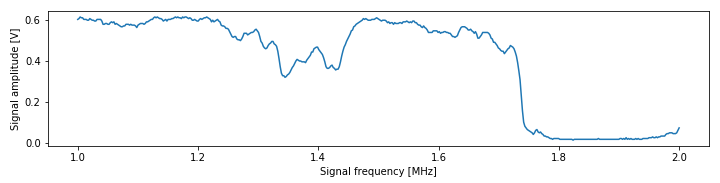
\includegraphics[width=\textwidth]{content/light-modulation/eom_strange.png}
}
\caption{The amplitude of the pockels cell depends on the repitition rate of the signal. The signal in this case was applying $0$, $V_\pi$, $0$ and $-V_\pi$ repeatedly.}
\end{figure}

The photodiode that is used is a home-built model, which has roughly a bandwidth of $\SI{22}{\mega \hertz}$. This is limiting the measurement of the rise time of the pockels cells, however it is possible to measure the extinction ratio. For this, the repitition rate is set to $\SI{200}{\kilo \hertz}$, where the amplitude is consistent. Measuring first the dark current of the photodiode and then taking the signal on the output of the beam splitter results in a extinction ratio of $>100:1$ as can be seen in Figure \ref{fig:eom_rtp_extc}.
\todo{do the diagram correctly}

\begin{figure}[h]
\label{fig:eom_rtp_extc}
\centering{
	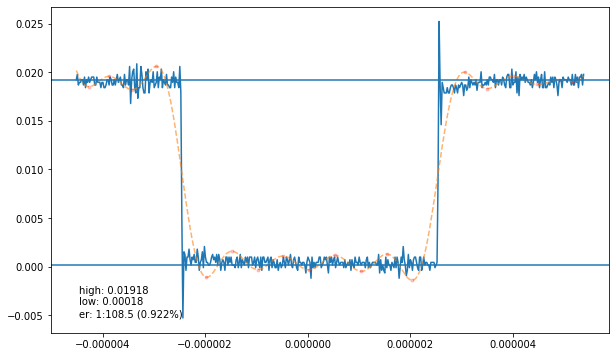
\includegraphics[width=\textwidth]{content/light-modulation/rtp_extc.png}
}
\caption{The \ac{rtp} pockels cell was driven with $\SI{200}{\kilo\hertz}$ at optimal beam parameters. By fitting a fourier series to the photodiode signal, it is possible to measure the extinction ratio, which is here $>100:1$. The peak at the beginning of the switching is an effect of the photodiode.}
\end{figure}

\todo{BBO}

\section{Acousto-optical modulators}
	\subsection{Operation}
	\subsection{Usage in the experiment}

